\documentclass[12pt]{article}

%%%% packages and definitions (optional)
\usepackage{graphicx} % allows inclusion of graphics
\usepackage{graphics}
\usepackage{placeins}
\usepackage{booktabs} % nice rules (thick lines) for tables
\usepackage{microtype} % improves typography for PDF
\usepackage{xspace}
\usepackage[hidelinks]{hyperref}
\usepackage{xspace}
\usepackage{hhline}
\usepackage{multirow}

\usepackage{varwidth}

\usepackage{rotating}
\usepackage[graphicx]{realboxes}
\usepackage{wrapfig}
\usepackage{lipsum}

\def\pgfcalendarweekdayletter#1{%  
 \ifcase#1M\or Tu\or W\or Tr\or F\or Sa\or Su\fi%  
}  
\usepackage{amsmath}

\usepackage{tabularx}
\newcolumntype{b}{>{\hsize=1.0\hsize}X}
\newcolumntype{s}{>{\hsize=.5\hsize}X}
\newcolumntype{m}{>{\hsize=.75\hsize}X}

\newcommand{\SN}{S$_N$}
\renewcommand{\vec}[1]{\bm{#1}} %vector is bold italic
\newcommand{\vd}{\bm{\cdot}} % slightly bold vector dot
\newcommand{\grad}{\vec{\nabla}} % gradient
\newcommand{\ud}{\mathop{}\!\mathrm{d}} % upright derivative symbol
\newcommand{\Cyclus}{\textsc{Cyclus}\xspace}%
\graphicspath{ {images/} }
\usepackage[affil-it]{authblk}
\usepackage[numbers]{natbib}
\usepackage{notoccite}
\usepackage{tikz}
\usetikzlibrary{positioning, arrows, decorations, shapes }
\usepackage{cleveref}

\usepackage{datatool}
\usepackage[acronym,toc]{glossaries}
%\newacronym{<++>}{<++>}{<++>}
\newacronym[longplural={metric tons of heavy metal}]{MTHM}{MTHM}{metric ton of heavy metal}
\newacronym{ABM}{ABM}{agent-based modeling}
\newacronym{ACDIS}{ACDIS}{Program in Arms Control \& Domestic and International Security}
\newacronym{ADS}{ADS}{Accelerator-Driven Systems}
\newacronym{AHTR}{AHTR}{Advanced High Temperature Reactor}
\newacronym{ANDRA}{ANDRA}{Agence Nationale pour la gestion des D\'echets RAdioactifs, the French National Agency for Radioactive Waste Management}
\newacronym{ANL}{ANL}{Argonne National Laboratory}
\newacronym{ANS}{ANS}{American Nuclear Society}
\newacronym{API}{API}{application programming interface}
\newacronym{ARE}{ARE}{Aircraft Reactor Experiment}
\newacronym{ARFC}{ARFC}{Advanced Reactors and Fuel Cycles}
\newacronym{ASME}{ASME}{American Society of Mechanical Engineers}
\newacronym{ATWS}{ATWS}{Anticipated Transient Without Scram}
\newacronym{BDBE}{BDBE}{Beyond Design Basis Event}
\newacronym{BIDS}{BIDS}{Berkeley Institute for Data Science}
\newacronym{BWR}{BWR}{Boiling Water Reactor}
\newacronym{CAFCA}{CAFCA}{ Code for Advanced Fuel Cycles Assessment }
\newacronym{CDTN}{CDTN}{Centro de Desenvolvimento da Tecnologia Nuclear}
\newacronym{CEA}{CEA}{Commissariat \`a l'\'Energie Atomique et aux \'Energies Alternatives}
\newacronym{CI}{CI}{continuous integration}
\newacronym{CNEN}{CNEN}{Comiss\~{a}o Nacional de Energia Nuclear}
\newacronym{CNERG}{CNERG}{Computational Nuclear Engineering Research Group}
\newacronym{COSI}{COSI}{Commelini-Sicard}
\newacronym{COTS}{COTS}{commercial, off-the-shelf}
\newacronym{CSNF}{CSNF}{commercial spent nuclear fuel}
\newacronym{CTAH}{CTAHs}{Coiled Tube Air Heaters}
\newacronym{CUBIT}{CUBIT}{CUBIT Geometry and Mesh Generation Toolkit}
\newacronym{CURIE}{CURIE}{Centralized Used Fuel Resource for Information Exchange}
\newacronym{DAG}{DAG}{directed acyclic graph}
\newacronym{DANESS}{DANESS}{Dynamic Analysis of Nuclear Energy System Strategies}
\newacronym{DBE}{DBE}{Design Basis Event}
\newacronym{DESAE}{DESAE}{Dynamic Analysis of Nuclear Energy Systems Strategies}
\newacronym{DHS}{DHS}{Department of Homeland Security}
\newacronym{DOE}{DOE}{Department of Energy}
\newacronym{DRACS}{DRACS}{Direct Reactor Auxiliary Cooling System}
\newacronym{DRE}{DRE}{dynamic resource exchange}
\newacronym{DSNF}{DSNF}{DOE spent nuclear fuel}
\newacronym{DYMOND}{DYMOND}{Dynamic Model of Nuclear Development }
\newacronym{EBS}{EBS}{Engineered Barrier System}
\newacronym{EDF}{EDF}{Électricité de France}
\newacronym{EDZ}{EDZ}{Excavation Disturbed Zone}
\newacronym{EIA}{EIA}{U.S. Energy Information Administration}
\newacronym{EPA}{EPA}{Environmental Protection Agency}
\newacronym{EPR}{EPR}{European Pressurized Reactor}
\newacronym{EP}{EP}{Engineering Physics}
\newacronym{EU}{EU}{European Union}
\newacronym{FCO}{FCO}{Fuel Cycle Options}
\newacronym{FCT}{FCT}{Fuel Cycle Technology}
\newacronym{FEHM}{FEHM}{Finite Element Heat and Mass Transfer}
\newacronym{FEPs}{FEPs}{Features, Events, and Processes}
\newacronym{FHR}{FHR}{Fluoride-Salt-Cooled High-Temperature Reactor}
\newacronym{FLiBe}{FLiBe}{Fluoride-Lithium-Beryllium}
\newacronym{FP}{FP}{Fission Products}
\newacronym{GDSE}{GDSE}{Generic Disposal System Environment}
\newacronym{GDSM}{GDSM}{Generic Disposal System Model}
\newacronym{GENIUSv1}{GENIUSv1}{Global Evaluation of Nuclear Infrastructure Utilization Scenarios, Version 1}
\newacronym{GENIUSv2}{GENIUSv2}{Global Evaluation of Nuclear Infrastructure Utilization Scenarios, Version 2}
\newacronym{GENIUS}{GENIUS}{Global Evaluation of Nuclear Infrastructure Utilization Scenarios}
\newacronym{GPAM}{GPAM}{Generic Performance Assessment Model}
\newacronym{GRSAC}{GRSAC}{Graphite Reactor Severe Accident Code}
\newacronym{GUI}{GUI}{graphical user interface}
\newacronym{HLW}{HLW}{high level waste}
\newacronym{HPC}{HPC}{high-performance computing}
\newacronym{HTC}{HTC}{high-throughput computing}
\newacronym{HTGR}{HTGR}{High Temperature Gas-Cooled Reactor}
\newacronym{IAEA}{IAEA}{International Atomic Energy Agency}
\newacronym{IEMA}{IEMA}{Illinois Emergency Mangament Agency}
\newacronym{IHLRWM}{IHLRWM}{International High Level Radioactive Waste Management}
\newacronym{INL}{INL}{Idaho National Laboratory}
\newacronym{IPRR1}{IRP-R1}{Instituto de Pesquisas Radioativas Reator 1}
\newacronym{IRP}{IRP}{Integrated Research Project}
\newacronym{ISFSI}{ISFSI}{Independent Spent Fuel Storage Installation}
\newacronym{ISRG}{ISRG}{Independent Student Research Group}
\newacronym{JFNK}{JFNK}{Jacobian-Free Newton Krylov}
\newacronym{LANL}{LANL}{Los Alamos National Laboratory}
\newacronym{LBNL}{LBNL}{Lawrence Berkeley National Laboratory}
\newacronym{LCOE}{LCOE}{levelized cost of electricity}
\newacronym{LDRD}{LDRD}{laboratory directed research and development}
\newacronym{LFR}{LFR}{Lead-Cooled Fast Reactor}
\newacronym{LLNL}{LLNL}{Lawrence Livermore National Laboratory}
\newacronym{LMFBR}{LMFBR}{Liquid Metal Fast Breeder Reactor}
\newacronym{LOFC}{LOFC}{Loss of Forced Cooling}
\newacronym{LOHS}{LOHS}{Loss of Heat Sink}
\newacronym{LOLA}{LOLA}{Loss of Large Area}
\newacronym{LP}{LP}{linear program}
\newacronym{LWR}{LWR}{Light Water Reactor}
\newacronym{MAGNOX}{MAGNOX}{Magnesium Alloy Graphie Moderated Gas Cooled Uranium Oxide Reactor}
\newacronym{MA}{MA}{minor actinide}
\newacronym{MCNP}{MCNP}{Monte Carlo N-Particle code}
\newacronym{MILP}{MILP}{mixed-integer linear program}
\newacronym{MIT}{MIT}{the Massachusetts Institute of Technology}
\newacronym{MOAB}{MOAB}{Mesh-Oriented datABase}
\newacronym{MOOSE}{MOOSE}{Multiphysics Object-Oriented Simulation Environment}
\newacronym{MOX}{MOX}{Mixed Oxide Fuel}
\newacronym{MSBR}{MSBR}{Molten Salt Breeder Reactor}
\newacronym{MSRE}{MSRE}{Molten Salt Reactor Experiment}
\newacronym{MSR}{MSR}{Molten Salt Reactor}
\newacronym{NAGRA}{NAGRA}{National Cooperative for the Disposal of Radioactive Waste}
\newacronym{NEAMS}{NEAMS}{Nuclear Engineering Advanced Modeling and Simulation}
\newacronym{NEUP}{NEUP}{Nuclear Energy University Programs}
\newacronym{NFCSim}{NFCSim}{Nuclear Fuel Cycle Simulator}
\newacronym{NGNP}{NGNP}{Next Generation Nuclear Plant}
\newacronym{NMWPC}{NMWPC}{Nuclear MW Per Capita}
\newacronym{NNSA}{NNSA}{National Nuclear Security Administration}
\newacronym{NPRE}{NPRE}{Department of Nuclear, Plasma, and Radiological Engineering}
\newacronym{NQA1}{NQA-1}{Nuclear Quality Assurance - 1}
\newacronym{NRC}{NRC}{Nuclear Regulatory Commission}
\newacronym{NSF}{NSF}{National Science Foundation}
\newacronym{NSSC}{NSSC}{Nuclear Science and Security Consortium}
\newacronym{NUWASTE}{NUWASTE}{Nuclear Waste Assessment System for Technical Evaluation}
\newacronym{NWF}{NWF}{Nuclear Waste Fund}
\newacronym{NWTRB}{NWTRB}{Nuclear Waste Technical Review Board}
\newacronym{OCRWM}{OCRWM}{Office of Civilian Radioactive Waste Management}
\newacronym{ORION}{ORION}{ORION}
\newacronym{ORNL}{ORNL}{Oak Ridge National Laboratory}
\newacronym{PARCS}{PARCS}{Purdue Advanced Reactor Core Simulator}
\newacronym{PBAHTR}{PB-AHTR}{Pebble Bed Advanced High Temperature Reactor}
\newacronym{PBFHR}{PB-FHR}{Pebble-Bed Fluoride-Salt-Cooled High-Temperature Reactor}
\newacronym{PEI}{PEI}{Peak Environmental Impact}
\newacronym{PH}{PRONGHORN}{PRONGHORN}
\newacronym{PRA}{PRA}{probabilistic risk assessment}
\newacronym{PRIS}{PRIS}{Power Reactor Information System}
\newacronym{PRKE}{PRKE}{Point Reactor Kinetics Equations}
\newacronym{PSPG}{PSPG}{Pressure-Stabilizing/Petrov-Galerkin}
\newacronym{PWAR}{PWAR}{Pratt and Whitney Aircraft Reactor}
\newacronym{PWR}{PWR}{Pressurized Water Reactor}
\newacronym{PyNE}{PyNE}{Python toolkit for Nuclear Engineering}
\newacronym{PyRK}{PyRK}{Python for Reactor Kinetics}
\newacronym{QA}{QA}{quality assurance}
\newacronym{RDD}{RD\&D}{Research Development and Demonstration}
\newacronym{RD}{R\&D}{Research and Development}
\newacronym{RELAP}{RELAP}{Reactor Excursion and Leak Analysis Program}
\newacronym{RIA}{RIA}{Reactivity Insertion Accident}
\newacronym{RIF}{RIF}{Region-Institution-Facility}
\newacronym{SFR}{SFR}{Sodium-Cooled Fast Reactor}
\newacronym{SINDAG}{SINDA{\textbackslash}G}{Systems Improved Numerical Differencing Analyzer $\backslash$ Gaski}
\newacronym{SKB}{SKB}{Svensk K\"{a}rnbr\"{a}nslehantering AB}
\newacronym{SNF}{SNF}{spent nuclear fuel}
\newacronym{SNL}{SNL}{Sandia National Laboratory}
\newacronym{STC}{STC}{specific temperature change}
\newacronym{SUPG}{SUPG}{Streamline-Upwind/Petrov-Galerkin}
\newacronym{SWF}{SWF}{Separations and Waste Forms}
\newacronym{SWU}{SWU}{Separative Work Unit}
\newacronym{TRIGA}{TRIGA}{Training Research Isotope General Atomic}
\newacronym{TRISO}{TRISO}{Tristructural Isotropic}
\newacronym{TSM}{TSM}{Total System Model}
\newacronym{TSPA}{TSPA}{Total System Performance Assessment for the Yucca Mountain License Application}
\newacronym{ThOX}{ThOX}{thorium oxide}
\newacronym{UFD}{UFD}{Used Fuel Disposition}
\newacronym{UML}{UML}{Unified Modeling Language}
\newacronym{UNF}{UNF}{Used Nuclear Fuel}
\newacronym{UOX}{UOX}{Uranium Oxide Fuel}
\newacronym{UQ}{UQ}{uncertainty quantification}
\newacronym{US}{US}{United States}
\newacronym{UW}{UW}{University of Wisconsin}
\newacronym{VISION}{VISION}{the Verifiable Fuel Cycle Simulation Model}
\newacronym{VVER}{VVER}{Voda-Vodyanoi Energetichesky Reaktor (Russian Pressurized Water Reactor)}
\newacronym{VV}{V\&V}{verification and validation}
\newacronym{WIPP}{WIPP}{Waste Isolation Pilot Plant}
\newacronym{YMR}{YMR}{Yucca Mountain Repository Site}

	
\makeglossaries

\title{Modeling Methods for Initiating Events in Nuclear Spent Fuel Repositories}
\author{Jin Whan Bae}
\affil{Dept. of Nuclear, Plasma, and Radiological Engineering, University of Illinois at Urbana-Champaign
		  Urbana, IL}
\date{}                     %% if you don't need date to appear
\setcounter{Maxaffil}{0}
\renewcommand\Affilfont{\itshape\small}
%%%%%%%%%%%%%%actual words%%%%%%%%%%%%%%%%%%%%%%%%%%%%%%%%%%%%%%%%%%%%%%%%%%%%5


\begin{document}
\maketitle

\section{Abstract}
\gls{UNF} repositories, given the high decay heat and radioactivity
of \glspl{UNF}, requires careful engineering. The current plan is
to design a repository that would contain the material for one million years.
Considering various events (failures) can occur in that time range,
the \gls{UNF} repository proposes an interesting subject for
\gls{PRA}. In this report, the model repository design is after the 
\gls{YMR}, which is a mined repository in volcanic tuff.
Ultimate failure status can be defined in various ways, depending on the
extent of leakage during the one million years (leakage from canister
\textasciitilde exposure to nearest population).
A definitive exposure of failure criteria must be defined,
in order for a reasonable analysis.  

Given the expansive
time range, very little real data is available.
Major issues or potential failures of the \gls{YMR} include volcanic activity
and canister failure. The two events have an extremely low
probability, but have catastrophic consequences. Considering that
risk is a function of both frequency and severity, the risk 
of the two factors is significant. Thus there is a necessity
to model the initiating events using non-traditional
risk analysis methods.

This project summarizes literature on methods of modeling
three initiating events of \gls{YMR}, and identifies
benefits and limitations of the methods. To clarify,
the word `modeling' in this report refers to initiating event
quantification, not identification.
Past research exists on 
modeling magma-drift interaction to predict volcanic and repository
failure events \cite{woods_modeling_2002},
using expert interpretation and opinion to measure epistemic
uncertainty of seismic activity probability \cite{stepp_probabilistic_2001}
and using a homogeneous Poisson process \cite{ho_risk_1992}.


\section{Background}
\gls{YMR} has been studied thoroughly in hopes of finally
disposing the U.S. \gls{UNF} inventory. However, considering
that it is a large project involving highly radioactive material,
careful planning and analyses must be done. The reference design
is taken from various sources \cite{u.s._department_of_energy_office_of_civilian_radioactive_waste_management_national_2008, wilson_total-system_1994, rechard_evolution_2014, u.s._department_of_energy_yucca_2002}.
Major sources of risk events are identified along with different ways to model
the events. 

Many risk events and components can be modeled using traditional methods like
failure probability from empirical tests and Human Reliability Analysis.
For simple mechanical procedures, for example, there exists previous data
on operation and failure probabilities. 

However, certain events are identified to be extremely difficult
to model using traditional risk analysis models. The events either
contain geological timescales or unpredictable natural disasters.
These events call for non-traditional methods of risk analysis.


\section{Literature Review}
System designs of the \gls{YMR} are listed extensively in literature \cite{u.s._department_of_energy_office_of_civilian_radioactive_waste_management_national_2008, wilson_total-system_1994, rechard_evolution_2014, u.s._department_of_energy_yucca_2002}, and contain multiple
iterations on the design. The basic design is as follows: the spent fuel assemblies
are repackaged in the waste package canister, and then placed underground,
underneath a drip shield. The canisters will remain there for up to millions of years,
surrounded by volcanic tuff.

Some prominent risk factors have also been identified. Volcanic hazards \cite{ho_risk_1992, smith_area_1990}
have been identified to be a long-term issue. Groundwater movement and transport of 
radioactive isotopes are another issue, in the case of canister breach \cite{robison_ground-water_1984, quade_fossil_1995}.  Canister reliability is another
identified risk factor \cite{whipple_can_1996, rutqvist_analysis_2003}.

Different aspects of risk analysis for nuclear waste repositories are published.
For systems where the future is hardly predictable, bayesian network analyses are 
suggested in \cite{lee_application_2006}. A method for sensitivity analysis
to rank important parameters are suggested in \cite{mohanty_cdf_2001}.


\section{Method}

Literature review will be done to study the methods of analyzing the three
initiating events - volcanic eruption, seismic activity and canister
corrosion. Studying the previous methods will bring insight into how
the initiating event works and how it affects the system of
interest (the repository). With the knowledge, limitations of
current methods and possible improvements are discussed.

\section{Definition of System Failure}
The definition of system failure depends on the scope of the system.
If the system is considered to be the entire repository, the `system failure' would be
`Radioactive Material Escape from Container.'
`Radioactive Material' would namely mean the spent fuel assemblies.
The container could be the transport cask which transports the assemblies from
the reactors to the site, or the emplacement cask, which is ultimately put in the repository.


\section{Definition of Initiating Event}
An initiating event is what causes a cascade of events that eventually leads
to the system failure, which is defined above as `Radioactive Material Escape
from Container'. 


\section{System Analysis}
To identify the initiating events to do literature review on,
we looked at various repository analyses and reports \cite{u.s._department_of_energy_office_of_civilian_radioactive_waste_management_national_2008, wilson_total-system_1994, rechard_evolution_2014, u.s._department_of_energy_yucca_2002},
in which many of them discuss the importance of geology and canister design.
In the case of the \gls{YMR}, seismic activity, volcanic eruption was considered
a structural concern. Additionally, like every repository, the integrity
of the container was a concern as well. Thus, the three events are chosen
as the object of this literature review.

Initiating events have been identified as crucial to the 
\gls{YMR} system are listed in table \ref{tab:ie}.
\begin{table}[h]
    \centering
%   \scalebox{0.86}{
        \begin{tabularx}{\linewidth}{mbb}
            \hline
            \textbf{Initiating Event} & \textbf{Reason} & \textbf{Difficulty to Model} \\ \hline
            \small{Volcanic Activity} & Repository rupture and Large Heat Influx & Rare event and needs modeling of physical phenomena \cite{marzocchi_quantifying_2004} \\ 
            \small{Canister Corrosion} & Leakage of Radioactive material & Modeling corrosion in geological time periods \cite{sadiq_probabilistic_2004, oldenburg_low-probability_2016} \\
            \small{Seismic Activity} & Repository rupture & Rare event and difficult to predict \cite{ward_multidisciplinary_1994} \\ \hline
        \end{tabularx}
        \caption{List of initiating events crucial to the failure of the \gls{YMR}}
        \label{tab:ie}
\end {table}

The three initiating events all have very little data
and cannot have empirical data to quantify their probabilities. Thus,
various methods have been used in an attempt to model these events.

\section{Goal}
The goal of this project is to research a method for effectively
modeling the three initiating events through literature review.
Preferably a value judgment will be made on the best method
for modeling the initiating event. 


\section{Volcanic Activity}
Yucca Mountain has been considered a potential site
for volcanic activity due to its multiple basalt centers 
of Quaternary age \cite{management_environmental_1986}.
Many papers \cite{crowe_volcanism:_2006, crowe_status_1995}claim that
the presence of those volcanic rocks are a result of early volcanic episodes in the region,
and that a volcanic activity is likely to occur.
There also is not a recorded volcanism near Yucca Mountain, which required
detailed volcanologic studies to be done to obtain the history of 
volcanic activity in the region.

\subsection{Simple Poisson Method}
The first attempt to calculate the probability of volcanic disruption
at Yucca Mountain was Crowe and Carr \cite{crowe_preliminary_1980}, using 
a simple Poisson model:
\[P_r = exp(-\lambda t p)\]
\[\lambda = \text{recurrence rate of volcanic events}\]
\[p = \text{probability of a repository disruption, given a volcanic eruption}\]

This model assumed three things:

\begin{enumerate}
    \item Volcanic eruptions in successive time periods are independent
     and should follow Poisson distribution with constant mean\\
    \item Every eruption has the same probability to disrupt the repository \\
    \item Disruption events are independent \\
\end{enumerate}

This model, using a refined mathematical model, resulted in a 
probability of volcanic disruption of the repository in the range of 
\textbf{3.3e-10 to 4.7e-8} for the first year, with a linear increase with time \cite{crowe_volcanic_1986}.

Though a brave feat, the Poisson model was not an adequate model for 
measuring a complex phenomenon like a volcanic eruption. The reasons
are the following:

\begin{enumerate}
    \item A simple Poisson model has a constant rate, which should be changing in time. Volcanic
            activities are considered "waning", "random", and "developing" in time \cite{ho_nonhomogeneous_1991}, meaning
            that the rate ($\lambda$) changes over time. 
    \item Clear understanding is needed of eruptive processes and reliable dating techniques.
\end{enumerate}


\subsection{Non-homogeneous Poisson Method}
An improvement from the simple Poisson model was made by using
non-homogeneous Poisson process with Weibull intensity \cite{ho_risk_1992}.
This process estimates the instantaneous recurrence rate using the
non-homogeneous Poisson process with Weibull intensity, and uses 
a homogeneous Poisson process to predict future eruptions.
Then, Bayesian analysis is performed to model the repository-disruptive frequency
given a volcanic eruption. This process replaces the constant $\lambda$ with
a time-dependent $\lambda(t)$. In the paper \cite{ho_risk_1992}, their choice of 
$\lambda(t)$ was the following:
\[ \lambda(t) = (\frac{t}{\theta})^{\beta}\]
which the first occurrenct follows a Weibull distribution, given by equation:
\[f(x;\lambda, k) = \frac{k}{\lambda} (\frac{x}{\lambda})^{k-1} for x\geq 0 \]

for different `stages', the $\beta$ holds different values, listed in table \ref{tab:beta}:

\begin{table}[h]
    \centering
%   \scalebox{0.86}{
        \begin{tabular}{cc}
            \hline
            \textbf{Volcano} & \textbf{$\beta$} \\ \hline
            Waning & 0.63 \\
            Random & 0.99 \\
            Developing & 5.40 \\
            \hline
       \end{tabular}
        \caption{Beta Values for different stages of volcanic period. If beta is larger than
                 1, the rate of eruption increases with time.}
        \label{tab:beta}
\end {table}

With the new $\lambda$ estimated, that $\lambda$ is plugged into simple Poisson distribution
(homogeneous Poisson) to calculate recurrence rate ($\lambda(t) t_0 $) for future time $[t, t+t_0]$.
This non-homogeneous Poisson method with updated eruption rate is to take into account both the 
specific physical events or processes that cause volcanic eruptions ($\lambda(t)$), and the 
various factors with random influences (Simple Poisson).

\begin{figure}[h]
\centering
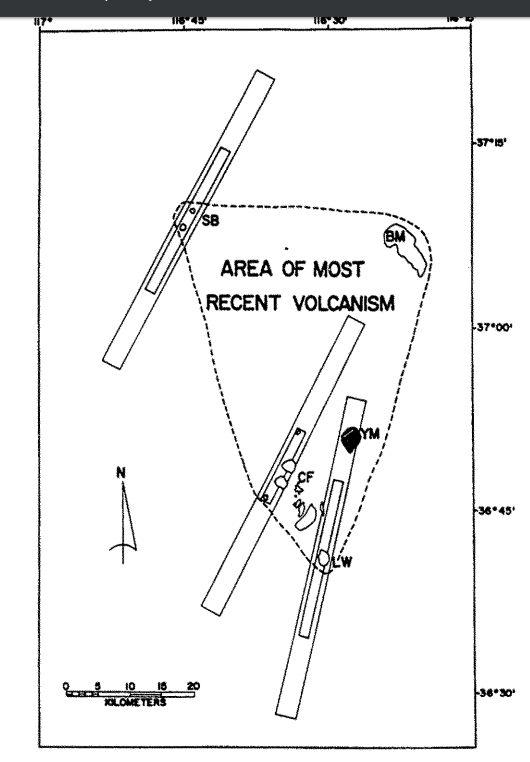
\includegraphics[scale=0.3]{./images/map.png}
\caption{This map outlines the are of most recent volcanic activity (dashed line)
and high-risk zones (rectangles). The dark shape labeled YM is the repository.}
\label{fig:map}
\end{figure}


For the probability of the volcanic eruption disrupting the repository, a map is drawn
with the area of most recent volcanic activity to identify high-risk zones (Figure \ref{fig:map}).
The proportion of the repository that is inside the risk zone is then used
for the upper limit for the probability.


The non-homogeneous Poisson method included various physical events and historic eruptions
into its risk calculation, as well as reflect the randomness of volcanic eruptions.
This resulted in a 90\% confidence interval for the probability of `site disruption'
of \textbf{0.01 to 0.067 for 10,000} years \cite{ho_risk_1992}.

\subsection{Multiple non-homogeneous Poisson models}
Connor et al. proposed a three non-homogeneous Poisson model
to model volcanic activity in Yucca Mountain \cite{connor_three_1995}.
The three methods are: spatio-temporal nearest neighbor,
kernel and nearest-neighbor kernel. The combination provides
the following benefits:
\begin{itemize}
    \item Recurrence rate and probability can be mapped \\
    \item No need to define areas of zones of volcanic activity \\
    \item Impact of uncertainty in timing and distribution is easy \\
\end{itemize}

This model incorporates more physical events and geological data 
in order to construct the three methods. The details of constructing 
the estimates with geological data (rock age, maps) is beyond the scope
of this review.

In short, this more detailed model takes into account the 
clustering of Quaternary volcanoes and the spatial dependency
or volcanic recurrence. This model resulted in a \textbf{ probability
of disruption within the 8 square kilometers of the repository
between 0.0001 and 0.0005 in 10,000 years} \cite{connor_three_1995}.


\subsection{Discussion}
The evolution of the methods of predicting volcanic eruption
and its probability to disrupt the repository was mainly
the evolution of taking into account various physical phenomenon
that change over time. Given geological timescales and lack
of historical data, predictions could only be made from current
geological formations that hint at a possibility of volcanic formation.
The reviewed papers progressively added layers and layers of geologic
and physical contribution to volcanic eruption, to add complexity to
their models.

Given a detailed geological database of the region and a clear understanding
of volcanic formation and activity, a Monte Carlo method can be an 
improvement from these multiple Poisson methods, where the entire
region can be simulated and tested to see if the repository is disrupted
in 10,000 years. However, such as feat would cost tremendous resources,
which would call for estimates and assumptions.  



\section{Canister Failure}
Canister failure is another modeling issue in nuclear repositories.
The science of corrosion and crack is well understood, but it is impossible
to run an experiment on a corrosion behavior for 100,000 years.
There have been various attempts to model this behavior and to measure
the probability of a canister failing. Depending on the
agency that performs these studies important material parameters, such
as pressure, temperature and atmosphere humidity differ. Thus, the main focus
of this section is on the method failure modeling and probability calculation.

\subsection{Empirical Correlation with Monte Carlo Simulation for Canister Corrosion}
To obtain a probability distribution function for the failure of a single
canister, the Sagar et al used a combination of empirical correlation
with Monte Carlo Simulation \cite{sagar_probabilistic_1986}.
Different empirical equations for discrete temperature regimes for 
small samples of material that was corroded for six weeks. The coefficients
of the equation are set as random variables with a normal distribution.
A Monte Carlo simulation is run to obtain the probability density
function for the failure probability of a container (result displayed in
figure \ref{fig:can}). Since the coefficient follows a normal distribution,
the probability density also resembles a normal distribution.

\begin{figure}[h]
\centering
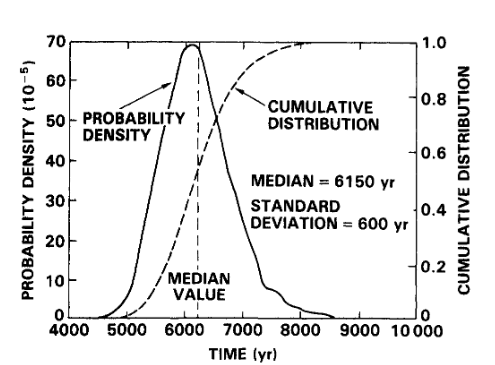
\includegraphics[scale=0.5]{./images/canister.png}
\label{fig:can}
\caption{Result of canister failure derived from Monte Carlo Simulation
         with empirical data.}
\end{figure}


\subsection{Material Testing with Monte Carlo Simulation for Canister Break}
The Swedish radioactive waste management company, or \gls{SKB}, 
performed extensive material testing with Monte Carlo method
to calculate the probability of canister failure. They performed
tensile test, compression tests, fracture mechanics tests as well 
as studied the microstructure of the canister material to obtain
the correlation of canister damage and defect. Using the data 
obtained from the experiments, they ran Monte Carlo simulations
on the failure probability given their geometry and pressure, to
obtain the probability of initiation of crack growth. 

\subsection{Discussion}
Canister failure, unlike volcanic activity, is a scientifically well
known and predictable event. The only difficulty lies on the 
uncertainty stemming from the long time period. Since it is unable
to perform thousand-year-long tests, most agencies use a combination
of shorter-term empirical measurement combined with a Monte-Carlo 
simulation to extend that correlation to a further future. However,
there are assumptions that the surrounding environment (pressure, humidty etc.)
will remain the same. An improvement can be made in which the surrounding environment
variables could be a distribution (or an equation with time, if possible)
that then creates a sample that the Monte Carlo simulation samples from.

\FloatBarrier


\section{Seismic Activity}

Seismic activity, similar to volcanic activity, is an initiating event
in the repository system that is difficult to model accurately. However,
earthquakes are more predictable than volcanic activities and can be 
analyzed in higher resolution. The discipline is well studied and 
established, and is called \gls{PSHA}.
The result of a \gls{PSHA} is the frequency of a seismic activity above
a certain threshold, or ``The rate of exceeding various ground-motion
levels at a site.'' \cite{thenhaus_seismic_2003}
 The \gls{PSHA} mostly takes the form of studying signs of seismic activity,
along with expert interpretation.
For example, Stepp et al. \cite{stepp_probabilistic_2001} studied the following categories
to predict earthquake probability in the Yucca Mountain region:
\begin{itemize}
    \item Faults within 100 km for Quaternary activity
    \item History and characteristics of past earthquake displacements  
    \item Contemporary earthquake activity
    \item Recorded earthquakes in the region
    \item Ground motion attnuation relationships
    \item Numerical modeling of ground motions from scenarios
\end{itemize}

The \gls{PSHA} is a combination of 
calculating the aleatory (random) uncertainty in
earthquake occurrence and the epistemic uncertainty
about the seismotectonic environment of a site.

\subsection{Aleatory Uncertainty in Earthquake Occurrence}

From the pioneering studies on \gls{PSHA} by \cite{mcguire_fortran_1976}
and \cite{cornell_engineering_1968}, the method for \gls{PSHA} 
is well-documented. First, the following inputs are obtained to calculate
the mean frequency of ground motion:

\begin{itemize}
    \item Seismic sources that contribute to site hazard 
    (probability distributions of distances of earthquake from site)
    \item Earthquake recurrence for each source 
    (mean annual rate of occurrence and magnitude distribution)
    \item Ground motion attenuation for region
\end{itemize}


The hazard calculation method integrates over the variables
to obtain the frequency of the earthquake. The hazard curve
is associated to each site. Each computed seismic hazard curve then
is combined into a logic tree, where each pathway is a conditional
probability of all the branches along the way. Thus, the result
is a family of hazard curves, with weights associated to each curve.



\subsection{Epistemic Uncertainty in Earthquake Occurrence}

Epistemic uncertainty was evaluated by a group of experts
who characterized seismic sources, fault displacement potentials
and ground motion attenuation in the region. The process 
was done with expert elicitation involving workshops,
consensus identification, and sharing of data and information.


\subsection{Summary and Discussion}
Many complex components go into the computation of 
seismic activity probability. The majority is the study
of geological survey and fault identification that allows
experts to determine the probability of a seismic activity.
The various parameters and expert interpretations are 
represented to a hazard curve, which is then collaborated
to a logic tree to find the probability of seismic activity
at the site of interest.
The validity (or the integrity) of the resulting frequency 
depends heavily on the thoroughness of the input parameters
and the expert interpretations. It is calculated in \cite{stepp_probabilistic_2001}
that the frequency for the \gls{YMR} site is $10^{-4}$/yr.



\section{Conclusion}

This paper lists the results of extensive literature
review on quantifying the frequency of seismic activity,
volcanic eruption, and canister failure in the \gls{YMR}.
For volcanic activity, the modeling improved by doing more
complex and multi-dimensional Poisson methods. For canister
failure, empirical correlations for short times are combined
with Monte-Carlo simulations to extrapolate to the far future.
For seismic activity, an already well-established \gls{PSHA}
combined analysis of potential seismic sources and historical
seismic activity data to model future seismic activity.


\section{Appendix - Reviewer Comments and Resolution}
The appendix includes comments from reviewers of the previously
submitted extended abstract.

\subsection{Reviewer 1 Comments and Resolution}

\textbf{Comments:}

\begin{center}
    \begin{varwidth}{0.8\textwidth}

`` The methods section is too broad – it states that initiating events that cannot be modeled are picked, however, seismic PRA methods have been developed for IEs of earthquakes. Exploration of volcanic IE is very interesting, this would be a neat topic for review. The ‘system analysis’ mentioned is also very vague, what is the system analysis method? It seems that the system analysis should result in a ranking? How can this ranking be connected to risk results? ''
    \end{varwidth}
\end{center}


\noindent \textbf{Resolution:}

The method section has been clarified to clearly define what will be
covered (probability/frequency quantification of three initiating events)
and how they will be covered (extensive literature review.)

For the system analysis, modifications are made to clarify the process
of how the author reached the conclusion of picking the three initiating 
events given the system under analysis. It follows a logic where various
\gls{YMR} reports and analyses are studied, and the author made a judgment
based on the reports that the three events were the most prevalent issues
in repository failure.

\subsection{Reviewer 2 Comments and Resolution:}


\textbf{Comments:}
\begin{center}
    \begin{varwidth}{0.8\textwidth}


`` 1) The term "modeling" needs to be clearly defined. When saying "Initiating Event (IE) analysis" in Probabilistic Risk Assessment (PRA), we usually refer to two aspects: IE Identification, and IE Quantification. In the final paper, please clarify the scope of “modeling” in this study; (2) Also, the word "system failure" (mentioned in Section 6) needs to be clarified. According to the contents under Section 6, it seems that an "end state" is defined as a combination of initiating event and system failure. For example, an earthquake (initiating event) occurs and leads to a crack in the cask (system failure), hence the radioactive material escapes from the cask to the environment (end state). Please provide this type of clarification in the final paper.''

    \end{varwidth}
\end{center}

\noindent \textbf{Resolution:}

1) A sentence was added saying the word `modeling' in this report refers to 
initiating event quantification, not identification. Identification
of the initiating events are already done by the author in the 
`system analysis' section.

2) The flexibility of the word `system failure', depending on the 
scope of the system,  is mentioned in the section defining system failure.

\subsection{Reviewer 3 Comments and Resolution:}

\textbf{Comments:}
\begin{center}
    \begin{varwidth}{0.8\textwidth}

``The topic is relevant to the PRA course. The level of sufficiency would depend on how much literature review is done for this work (e.g., number of references to be analyzed), as apparently the author does not include quantitative PRA analysis (e.g., event tree, fault tree) in the schedule. In the final paper, it is suggested that difficulties in modeling the initiating events of interest be justified by elaborating the literature review to find out what the challenges are and reasons for those challenges. Table 1 given in the extended abstract needs to be justified (and acknowledged) by adding references from different domains, not just from the nuclear industry. ''

    \end{varwidth}
\end{center}

\noindent \textbf{Resolution:}

Other papers from other domains are reviewed and added in the paper
as citations next to Table 1.


\pagebreak 



\bibliographystyle{unsrtnat}
\bibliography{bibliography}


\end{document}
\grid
